\chapter{Diseño e implementación}
\label{Chapter3}
\begingroup\sloppy\setlength{\emergencystretch}{2.5em}

En el presente capítulo se describe el diseño e implementación del sistema de detección de anomalías: el pipeline de datos desde Prometheus hasta las ventanas multivariadas, la arquitectura del autoencoder LSTM, el procedimiento de entrenamiento y calibración del umbral, y la integración del servicio de inferencia con Opsgenie y Grafana.

\begin{figure}[H]
\centering
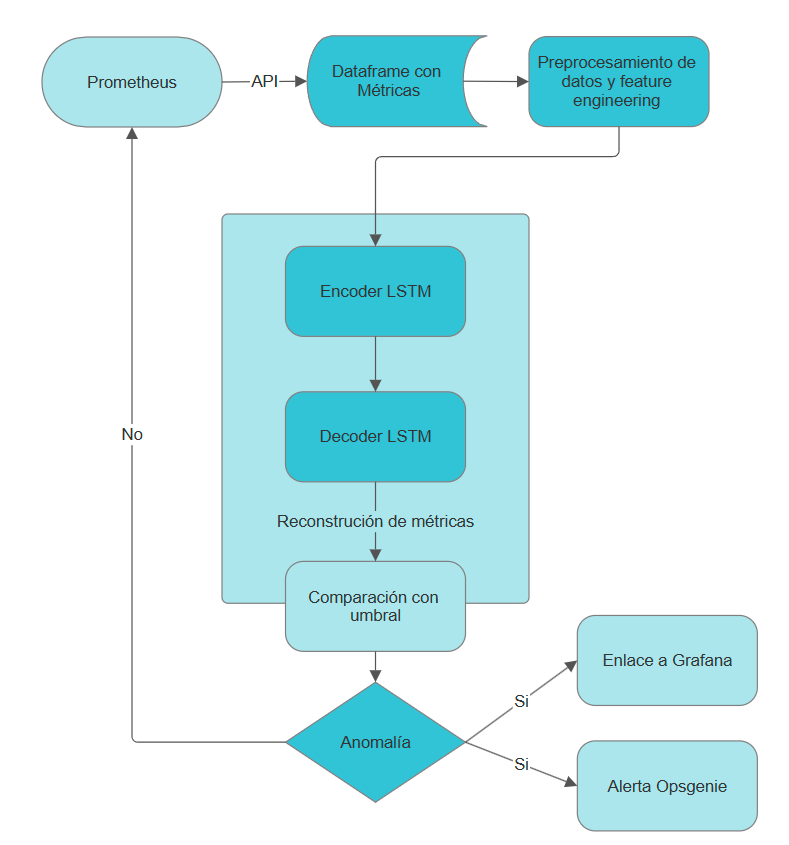
\includegraphics[width=0.95\textwidth]{./Figures/flow_diag.png}
\caption{Flujo del sistema de detección: desde Prometheus hasta alertas en Opsgenie y enlace contextual a Grafana.}
\label{fig:flujo-sistema}
\end{figure}

La figura~\ref{fig:flujo-sistema} resume el flujo operativo completo, desde la recolección de telemetría hasta la emisión de alertas contextualizadas.

\section{Pipeline de datos}
\label{sec:pipeline-datos}

El pipeline de datos automatiza las etapas que transforman telemetría cruda en secuencias listas para el modelo. 

Se implementó como un conjunto de módulos Python invocados desde el script de entrenamiento (\filepath{scripts/train.py}) y reutilizados en inferencia (\filepath{scripts/inference.py}), de modo que entrenamiento y producción comparten exactamente las mismas reglas de transformación.

La configuración operativa, incluidas las consultas PromQL, las cotas de normalización, el tamaño de ventana y los parámetros de alerta, se externalizó en archivos YAML bajo \filepath{config/}, lo que permitió ajustar el comportamiento sin modificar el código fuente.

\subsection{Recolección y alineación temporal}

La primera etapa obtiene series desde la API HTTP de rango de Prometheus (\filepath{api/v1/query\_range}).

Un cliente dedicado (\texttt{PrometheusClient}) lee las consultas definidas en \filepath{config/data.yaml} y ejecuta cada consulta con paso de muestreo de 30~segundos.

Tras obtener las series por instancia, se agregaron los resultados según la semántica de cada métrica:

\begin{itemize}
\item \texttt{sum}: contadores y tasas (\texttt{request\_rate}, \texttt{error\_rate}, \texttt{cpu\_usage}).
\item \texttt{max}: percentiles de latencia (\texttt{latency\_p95}).
\item \texttt{mean}: gauges de memoria (\texttt{memory\_usage}).
\end{itemize}

Las series devueltas se integraron en un marco temporal común, con \texttt{timestamp} como índice.

Cuando faltaban puntos aislados dentro del intervalo de muestreo, se aplicó forward-fill acotado antes de descartar ventanas incompletas. El cliente incorporó además un ajuste automático del paso de consulta cuando el rango solicitado superaba el límite de 11\,000 puntos por petición impuesto por Prometheus y preservó la cobertura temporal sin truncar silenciosamente el historial.

Para el entrenamiento sobre el entorno autorizado de la empresa, el cliente apuntó a la instancia Prometheus interna. En el repositorio reproducible y en el perfil \texttt{dev} de Docker Compose, las mismas consultas se ejecutaron contra un servicio simulado instrumentado con \filepath{prometheus\_client}, compartiendo núcleo de generación con el generador sintético offline (\filepath{traffic\_simulation\_core.py}).

Así se garantizó paridad semántica entre fuentes sin exponer telemetría confidencial en el material académico reproducible.

La tabla~\ref{tab:promql-queries} detalla las consultas PromQL configuradas, la agregación aplicada tras obtener las series por instancia y la interpretación operativa de cada señal. Mantener las consultas declarativas permitió auditar qué aspecto del servicio alimenta cada variable del modelo y replicar el mismo criterio en el simulador.

\begin{table}[H]
\centering
\footnotesize
\caption{Consultas PromQL y agregación por métrica del servicio.}
\label{tab:promql-queries}
\begin{tabular}{@{}>{\raggedright\arraybackslash}p{0.18\textwidth}>{\raggedright\arraybackslash}p{0.44\textwidth}cp{0.22\textwidth}@{}}
\toprule
\textbf{Variable} & \textbf{Consulta PromQL (resumida)} & \textbf{Agreg.} & \textbf{Interpretación} \\
\midrule
\texttt{request\_rate} & \texttt{rate(http\_requests\_\allowbreak total[5m])} & sum & Demanda instantánea sobre el servicio \\
\texttt{latency\_p95} & \texttt{histogram\_quantile(0.95,}\allowbreak\texttt{ rate(...[5m]))} & max & Cola superior de tiempos de respuesta \\
\texttt{memory\_usage} & \texttt{process\_resident\_\allowbreak memory\_bytes\{...\}} & mean & Presión de memoria del proceso \\
\texttt{error\_rate} & \texttt{rate(http\_request\_\allowbreak errors\_total[5m])} & sum & Tasa de respuestas erróneas \\
\texttt{cpu\_usage} & \texttt{rate(process\_cpu\_\allowbreak seconds\_total[5m])} & sum & Consumo de CPU del servicio \\
\bottomrule
\end{tabular}
\end{table}

El intervalo de cinco minutos en las funciones \texttt{rate} y \texttt{histogram\_quantile} suavizó fluctuaciones de muestreo periódico sin ocultar degradaciones sostenidas. Ese valor se mantuvo coherente con las reglas de alerta existentes en la organización, lo que facilitó contrastar el detector aprendido con umbrales declarativos en evaluaciones posteriores.

Cuando el historial solicitado superaba el límite de puntos por consulta, el cliente recalculó el paso efectivo manteniendo fijo el rango temporal total. De este modo, un entrenamiento sobre 90~días no truncó silenciosamente las primeras semanas del período, situación que se detectó en pruebas iniciales y que habría sesgado la estimación de estacionalidad semanal. La resolución efectiva resultante fue más gruesa solo cuando fue estrictamente necesaria para cumplir la restricción de la API.

Se eligió un horizonte de 90~días porque cubre varios ciclos semanales completos y proporciona del orden de 259\,200 muestras por métrica, volumen suficiente para estimar un régimen nominal estable sin exigir almacenamiento excesivo. El particionado reservó el 20~\% final de las ventanas para validación y preservó el orden cronológico a fin de evitar filtraciones de información futura. Las cinco métricas técnicas y las variables temporales derivadas se caracterizaron en la sección~\ref{sec:datasets}.

\subsection{Ingeniería de variables y normalización}

Tras la alineación, el módulo \texttt{DataPreprocessor} enriqueció cada instante con seis variables temporales derivadas del reloj de la muestra:

\begin{enumerate}
\item \texttt{hour\_sin} y \texttt{hour\_cos}: codificación cíclica de la hora del día mediante $\sin(2\pi h/24)$ y $\cos(2\pi h/24)$.
\item \texttt{dayofweek\_sin} y \texttt{dayofweek\_cos}: codificación cíclica del día de la semana ($0$--$6$).
\item \texttt{is\_weekend}: indicador binario para sábado y domingo.
\item \texttt{is\_night}: indicador binario para el intervalo 22:00--06:00.
\end{enumerate}

La codificación cíclica evita discontinuidades artificiales en los límites del calendario (por ejemplo, entre las 23:00 y las 00:00) y permite al modelo distinguir patrones diarios y semanales sin depender de umbrales fijos por horario.

La normalización se realizó con \texttt{MinMaxScaler} en modo \texttt{fixed\_minmax}: en lugar de ajustar mínimos y máximos sobre el conjunto de entrenamiento, se fijaron cotas determinísticas por variable en \filepath{config/data.yaml}, derivadas del análisis del servicio simulado y validadas contra consultas reales. La tabla~\ref{tab:fixed-bounds} resume los rangos adoptados.

En las primeras iteraciones se probó \texttt{StandardScaler}, que memoriza media y desviación estándar del lote de entrenamiento. Cuando el modelo entrenado con datos sintéticos se evaluó sobre Prometheus productivo, las series normalizadas quedaron desplazadas respecto del dominio aprendido y el error de reconstrucción superó el umbral de forma sistemática en tramos nominales.

El modo \texttt{fixed\_minmax} eliminó ese acoplamiento: la misma observación cruda produce siempre la misma coordenada normalizada, con independencia del origen o del período de entrenamiento. Este criterio resultó central para desplegar un único par modelo--preprocesador en producción sin recalibrar el escalador ante cada reentrenamiento.

\begin{table}[H]
\centering
\footnotesize
\caption{Cotas de normalización \texttt{fixed\_minmax} por variable.}
\label{tab:fixed-bounds}
\begin{tabular}{@{}p{0.32\textwidth}p{0.28\textwidth}p{0.32\textwidth}@{}}
\toprule
\textbf{Variable} & \textbf{Rango mínimo} & \textbf{Rango máximo} \\
\midrule
\texttt{request\_rate} & 0 req/s & 150 req/s \\
\texttt{latency\_p95} & 0 s & 0,50 s \\
\texttt{memory\_usage} & 0 B & $2 \times 10^9$ B \\
\texttt{error\_rate} & 0 err/s & 3,0 err/s \\
\texttt{cpu\_usage} & 0 & 0,15 \\
Variables temporales cíclicas & $-1$ & 1 \\
Indicadores binarios & 0 & 1 \\
\bottomrule
\end{tabular}
\end{table}

El preprocesador serializado (\filepath{models/preprocessor.joblib}) persiste el escalador, la lista de columnas activas y la configuración de variables temporales, de modo que inferencia y entrenamiento aplican la misma transformación bit a bit.

Las cotas de la tabla~\ref{tab:fixed-bounds} se derivaron del análisis del servicio simulado: la tasa de peticiones sigue un factor diario sinusoidal con ruido gaussiano, la latencia percentil 95 se modela como proporcional a ese factor más un piso constante, y las tasas de error y CPU escalan con la demanda esperada. Los límites superiores incorporaron margen por encima del máximo observado en condiciones nominales para absorber picos breves sin saturar la escala. Si una observación excediera una cota, \texttt{MinMaxScaler} la acotó al intervalo $[0,1]$, señal explícita de régimen extremo que el autoencoder aprendió a reconstruir con mayor error.

\subsection{Construcción de ventanas deslizantes}

La etapa final del pipeline convirtió la serie multivariada preprocesada en tensores tridimensionales $(N, T, F)$, donde $N$ es la cantidad de ventanas, $T = 20$ el número de pasos temporales y $F = 11$ el número de variables por paso. La clase \texttt{WindowGenerator} implementó dos modos:

\begin{itemize}
\item Entrenamiento (\texttt{create\_sequences}): ventanas deslizantes con \textit{stride}~$= 1$, con solapamiento máximo entre muestras consecutivas. Con 90~días de muestreo cada 30~segundos, ello generó del orden de $250\,000$ ventanas, frente a unas $12\,000$ obtenidas con stride~$= 20$ en prototipos iniciales.
\item Inferencia (\texttt{create\_single\_window}): extracción de los últimos $T$ puntos disponibles. Si la cantidad era insuficiente, el servicio omitía el ciclo de detección en lugar de rellenar con ceros, para evitar falsos positivos por ventanas artificialmente completadas.
\end{itemize}

Cada ventana abarcó 10~minutos de operación ($20 \times 30\,\mathrm{s}$), horizonte elegido por equilibrar sensibilidad a degradaciones sostenidas y costo de cómputo en CPU. El particionado entre entrenamiento y validación reservó el 20~\% final de las ventanas y preservó el orden cronológico.

La longitud de 20 pasos implicó que una anomalía puntual de un solo muestreo quedara diluida en la reconstrucción global de la ventana, mientras que desvíos sostenidos durante varios minutos, el caso operativo de interés, modificaron de forma coherente múltiples pasos y varias variables a la vez y elevaron el error agregado por encima del umbral. Ventanas más cortas (10 pasos) reaccionaron antes pero fueron más sensibles al ruido. Ventanas de 30 pasos (15~minutos) suavizaron en exceso incidentes breves. El valor 20 resultó del benchmark interno documentado en \filepath{tune\_model.py}.

La tabla~\ref{tab:pipeline-etapas} detalla entradas, salidas y artefactos de cada etapa.

\begin{table}[H]
\centering
\small
\caption{Etapas del pipeline de datos y artefactos producidos.}
\label{tab:pipeline-etapas}
\begin{tabular}{@{}p{0.22\textwidth}p{0.34\textwidth}>{\raggedright\arraybackslash}p{0.34\textwidth}@{}}
\toprule
\textbf{Etapa} & \textbf{Entrada / salida} & \textbf{Implementación} \\
\midrule
Recolección & Consultas PromQL $\rightarrow$ series por métrica & \texttt{PrometheusClient}, \filepath{config/data.yaml} \\
Alineación & Series $\rightarrow$ marco temporal unificado & \texttt{pandas}, forward-fill acotado \\
Ingeniería & Marco + reloj $\rightarrow$ 11 variables & \filepath{DataPreprocessor.\_add\_temporal\_features} \\
Normalización & Valores crudos $\rightarrow$ $[0,1]$ fijo & \texttt{MinMaxScaler} con cotas en YAML \\
Ventanas & Serie $\rightarrow$ $(N, 20, 11)$ & \texttt{WindowGenerator} \\
Persistencia & Escalador y metadatos & \filepath{preprocessor.joblib} \\
\bottomrule
\end{tabular}
\end{table}

\subsection{Organización del código fuente}

El repositorio entregable agrupó la lógica en cuatro paquetes bajo \filepath{src/}, más scripts ejecutables en \filepath{scripts/} y configuración en \filepath{config/}. La tabla~\ref{tab:modulos} resume la responsabilidad de cada módulo principal. Esta separación permitió probar el preprocesamiento y la generación de ventanas de forma aislada antes de integrarlos con el servicio de inferencia.

\begin{table}[H]
\centering
\footnotesize
\caption{Módulos implementados y responsabilidad funcional.}
\label{tab:modulos}
\begin{tabular}{@{}>{\raggedright\arraybackslash}p{0.34\textwidth}>{\raggedright\arraybackslash}p{0.56\textwidth}@{}}
\toprule
\textbf{Módulo / script} & \textbf{Responsabilidad} \\
\midrule
\filepath{src/data/prometheus\_client.py} & Consultas HTTP, agregación y alineación de series \\
\filepath{src/data/preprocessor.py} & Variables temporales y normalización \\
\filepath{src/data/windowing.py} & Ventanas deslizantes para entrenamiento e inferencia \\
\filepath{src/data/synthetic\_data.py} & Generación offline de series de respaldo \\
\filepath{src/models/lstm\_autoencoder.py} & Definición, entrenamiento y persistencia del modelo \\
\filepath{src/alerting/detector.py} & Puntuación de anomalía por ventana \\
\filepath{src/alerting/opsgenie\_client.py} & Emisión de alertas y notificaciones de resolución \\
\filepath{src/alerting/grafana\_links.py} & Construcción de URLs contextuales al panel de Grafana \\
\filepath{scripts/train.py} & Orquestación del entrenamiento extremo a extremo \\
\filepath{scripts/inference.py} & Bucle de detección en tiempo de operación \\
\filepath{scripts/tune\_model.py} & Exploración de arquitecturas sin afectar artefactos productivos \\
\bottomrule
\end{tabular}
\end{table}

\subsection{Paridad entre entrenamiento e inferencia}

Un requisito no funcional central del diseño fue garantizar que una ventana procesada en producción fuera indistinguible, desde el punto de vista del modelo, de una ventana equivalente obtenida durante el entrenamiento.

Cualquier divergencia en el orden de transformaciones, en las columnas activas o en la política de ventanas se tradujo en errores de reconstrucción artificialmente elevados y en falsos positivos masivos, fenómeno reproducido al comparar un escalado adaptativo entrenado con datos sintéticos contra consultas reales a Prometheus.

Para cerrar esa brecha se adoptaron tres medidas concretas.

Primero, el mismo objeto \texttt{DataPreprocessor} serializado se cargó en inferencia sin reajuste sobre datos recientes. Segundo, las consultas PromQL y las reglas de agregación se leyeron del mismo archivo \filepath{config/data.yaml} en ambos modos. Tercero, la generación de ventanas en inferencia utilizó exclusivamente los últimos $T$ puntos completos, mientras que en entrenamiento se generó el conjunto completo con stride~$=1$, pero aplicando la misma función de extracción por ventana.

La tabla~\ref{tab:train-inferencia-paridad} contrasta el comportamiento en cada fase. Las diferencias restantes son intencionales: el solapamiento masivo solo tiene sentido offline para aumentar muestras de entrenamiento, mientras que en línea basta la ventana corriente.

\begin{table}[H]
\centering
\small
\caption{Paridad y diferencias deliberadas entre entrenamiento e inferencia.}
\label{tab:train-inferencia-paridad}
\begin{tabular}{@{}>{\raggedright\arraybackslash}p{0.24\textwidth}>{\raggedright\arraybackslash}p{0.30\textwidth}>{\raggedright\arraybackslash}p{0.32\textwidth}@{}}
\toprule
\textbf{Aspecto} & \textbf{Entrenamiento} & \textbf{Inferencia} \\
\midrule
Fuente de datos & 90~días históricos & Últimos 10~minutos \\
Consultas PromQL & \filepath{config/data.yaml} & Mismo archivo \\
Preprocesador & \texttt{fit\_transform} + persistencia & \texttt{load} + \texttt{transform} \\
Generación de ventanas & \texttt{create\_\allowbreak sequences}, stride~$=1$ & \texttt{create\_\allowbreak single\_window} \\
Ventana incompleta & Descartada al particionar & Omite ciclo (sin relleno) \\
Salida del modelo & Pérdida MSE + umbral & Error $e$ vs.\ $\tau$ + alerta \\
\bottomrule
\end{tabular}
\end{table}

\section{Arquitectura del modelo}
\label{sec:arquitectura-modelo}

El núcleo analítico es un autoencoder LSTM secuencia a secuencia: aprende a comprimir una ventana nominal en una representación latente y a reconstruirla paso a paso. En inferencia, un error de reconstrucción elevado indica que la ventana observada no coincide con los patrones aprendidos durante el entrenamiento sobre tramos nominales. La figura~\ref{fig:flujo-sistema} sitúa este componente dentro del flujo global del sistema, desde la recolección en Prometheus hasta la emisión de alertas.

\subsection{Codificador y decodificador}

La arquitectura implementada en \texttt{LSTMAutoencoder} (\filepath{src/models/lstm\_autoencoder.py}) siguió el esquema codificador--bottleneck--decodificador de Malhotra et al. \citep{malhotra2015long}, adaptado al vector de once variables y a la ventana de 20 pasos.

El codificador apiló tres capas \texttt{LSTM} con 64, 32 y 16 unidades respectivamente. Las dos primeras devolvieron secuencias completas (\texttt{return\_sequences=True}), y la tercera produjo el vector latente de dimensión 16. Entre capas recurrentes se insertó \textit{dropout} del 10~\% para regularizar.

El decodificador expandió el latente mediante \texttt{RepeatVector}, replicándolo a lo largo de los 20 pasos temporales, y aplicó tres capas \texttt{LSTM} simétricas (16, 32 y 64 unidades) con dropout del 10~\%. La salida se obtuvo con una capa \texttt{TimeDistributed}\allowbreak\texttt{(Dense(11))} que reconstruyó las once variables en cada instante.

La tabla~\ref{tab:capas-modelo} resume la pila de capas, formas tensoriales intermedias y justificación de diseño.

\begin{table}[H]
\centering
\small
\caption{Capas del autoencoder LSTM y formas intermedias ($B$ = tamaño de lote).}
\label{tab:capas-modelo}
\begin{tabular}{@{}p{0.24\textwidth}cp{0.48\textwidth}@{}}
\toprule
\textbf{Capa} & \textbf{Forma de salida} & \textbf{Rol} \\
\midrule
Entrada & $(B, 20, 11)$ & Ventana multivariada normalizada \\
LSTM codificador 64 & $(B, 20, 64)$ & Captura dependencias locales \\
LSTM codificador 32 & $(B, 20, 32)$ & Compresión progresiva \\
LSTM codificador 16 & $(B, 16)$ & Representación latente \\
RepeatVector & $(B, 20, 16)$ & Expansión temporal del latente \\
LSTM decodificador 16--64 & $(B, 20, 64)$ & Reconstrucción secuencial \\
Dense por paso & $(B, 20, 11)$ & Salida reconstruida \\
\bottomrule
\end{tabular}
\end{table}

\subsection{Función de pérdida y señal de anomalía}

El entrenamiento minimizó el error cuadrático medio (MSE) \citep{chollet2015keras} entre la ventana de entrada y su reconstrucción, promediado sobre los 20 pasos y las 11 variables. Como métrica auxiliar de monitoreo se registró el error absoluto medio (MAE) \citep{chollet2015keras}. En inferencia, la señal escalar de anomalía fue el MSE por ventana, definido en la ecuación~\eqref{eq:mse-reconstruccion}:
\begin{equation}
e = \frac{1}{T \cdot F} \sum_{t=1}^{T} \sum_{f=1}^{F} \bigl(x_{t,f} - \hat{x}_{t,f}\bigr)^2
\label{eq:mse-reconstruccion}
\end{equation}
donde $x$ es la ventana observada y $\hat{x}$ la reconstrucción del modelo. Una ventana se marcó como anómala cuando $e$ superó un umbral $\tau$ calibrado sobre errores de validación (sección~\ref{sec:entrenamiento}).

Además del criterio binario, se definió una magnitud de confianza relativa para priorizar alertas, según la ecuación~\eqref{eq:confianza-anomalia}:
\begin{equation}
c = \frac{e - \tau}{\tau} \quad \text{cuando } e > \tau
\label{eq:confianza-anomalia}
\end{equation}
y $c = 0$ en caso contrario. Valores de $c$ más altos indicaron un apartamiento más marcado del régimen nominal aprendido.

\begin{table}[H]
\centering
\small
\caption{Asignación de prioridad Opsgenie según confianza de la anomalía.}
\label{tab:opsgenie-prioridad}
\begin{tabular}{@{}ccp{0.46\textwidth}@{}}
\toprule
\textbf{Prioridad} & \textbf{Umbral de $c$} & \textbf{Interpretación operativa} \\
\midrule
P1 & $c > 2{,}0$ & Desvío muy marcado. Respuesta inmediata \\
P2 & $c > 1{,}0$ & Degradación significativa. Escalamiento si persiste \\
P3 & $c > 0{,}5$ & Anomalía moderada. Revisión en guardia \\
P4 & $c \leq 0{,}5$ & Registro sin escalamiento urgente \\
\bottomrule
\end{tabular}
\end{table}

Esos valores se utilizaron para asignar prioridad en Opsgenie (tabla~\ref{tab:opsgenie-prioridad}).

\subsection{Acoplamiento multivariado y espacio latente}

A diferencia de reglas univariadas por métrica, el autoencoder procesa las once variables de forma conjunta en cada paso temporal. El codificador LSTM mantiene un estado oculto que acumula contexto a lo largo de los 20 pasos, de modo que una subida aislada de latencia en presencia de demanda estable y error nulo puede reconstruirse con bajo error, mientras que una combinación de incremento simultáneo en \texttt{error\_rate}, \texttt{latency\_p95} y \texttt{cpu\_usage} eleva $e$ aunque ninguna variable supere por sí sola un umbral fijo predefinido.

El vector latente de dimensión 16 actúa como \textit{bottleneck}: obliga al modelo a capturar regularidades compactas del régimen nominal (ciclos diarios, diferencia fin de semana vs.\ día hábil, correlación entre carga y latencia) y descartar variaciones de alta frecuencia no repetibles. Durante el entrenamiento, la pérdida de validación descendió de forma monótona hasta estabilizarse en valores del orden de $10^{-3}$ en la escala normalizada, señal de que el bottleneck conservó información suficiente para reconstruir ventanas nominales sin memorizar ruido puntual. La tabla~\ref{tab:complejidad-modelo} resume la complejidad paramétrica y el costo operativo.

\begin{table}[H]
\centering
\small
\caption{Complejidad del modelo y costo operativo estimado.}
\label{tab:complejidad-modelo}
\begin{tabular}{@{}p{0.38\textwidth}p{0.48\textwidth}@{}}
\toprule
\textbf{Atributo} & \textbf{Valor o estimación} \\
\midrule
Parámetros entrenables & Del orden de $10^5$ (capas LSTM + densas) \\
Entrada por inferencia & 1 ventana $(20, 11)$ \\
Tiempo por ciclo de detección & $< 1$~s en contenedor con 1 vCPU \\
Memoria del contenedor de detección & Límite 2~GB. Uso típico inferior a 512~MB \\
Frecuencia del bucle & 1 evaluación cada 30~s \\
\bottomrule
\end{tabular}
\end{table}

\subsection{Decisiones de diseño arquitectónico}

Se eligió una topología simétrica 64--32--16--32--64 por ser suficientemente expresiva para once variables en CPU y mantener tiempos de inferencia acotados (inferior a un segundo por ciclo en el contenedor de despliegue). Configuraciones con bottleneck más estrecho (8 unidades) y más ancho (32 unidades) se evaluaron en el script \filepath{tune\_model.py}. La topología base ofreció el mejor equilibrio entre pérdida de validación y estabilidad frente a datos de Prometheus.

La activación lineal en la capa de salida preservó la interpretabilidad de las variables reconstruidas en la escala normalizada. No se emplearon capas convolucionales ni mecanismos de atención: el muestreo fijo cada 30~segundos y la ventana corta de 10~minutos hicieron innecesaria una mayor complejidad para capturar la estacionalidad diaria modelada explícitamente mediante variables temporales.

Los pesos entrenados y la configuración estructural se serializaron por separado (\filepath{lstm\_autoencoder.weights.h5} y \filepath{lstm\_autoencoder\_config.json}) para reconstruir el grafo computacional en inferencia sin acoplarse a una versión concreta del entorno de entrenamiento.

\section{Entrenamiento y optimización}
\label{sec:entrenamiento}

Esta sección documenta el procedimiento de entrenamiento del autoencoder, la calibración del umbral de detección y la exploración acotada de hiperparámetros alternativos.

\subsection{Procedimiento de entrenamiento}

El script \filepath{scripts/train.py} orquestó el flujo completo: carga de configuración, obtención de datos, preprocesamiento, generación de ventanas, entrenamiento, persistencia de artefactos y cálculo del umbral. Los hiperparámetros principales se fijaron en \filepath{config/model.yaml} y se resumen en la tabla~\ref{tab:hiperparametros}.

\begin{table}[H]
\centering
\small
\caption{Hiperparámetros de entrenamiento del autoencoder LSTM.}
\label{tab:hiperparametros}
\begin{tabular}{@{}p{0.38\textwidth}p{0.48\textwidth}@{}}
\toprule
\textbf{Parámetro} & \textbf{Valor} \\
\midrule
Optimizador & Adam, tasa de aprendizaje 0,001 \\
Función de pérdida & MSE \\
Tamaño de lote (\textit{batch}) & 256 \\
Épocas máximas & 30 \\
Parada temprana & Paciencia 10 épocas sobre \texttt{val\_loss} \\
Reducción de tasa de aprendizaje & Factor 0,5 cuando \texttt{val\_loss} se estanca \\
Partición entrenamiento / validación & 80~\% / 20~\% temporal \\
Dropout entre capas LSTM & 0,1 \\
\bottomrule
\end{tabular}
\end{table}

El optimizador Adam actualizó los pesos minimizando la MSE entre entrada y salida del autoencoder (objetivo clásico de reconstrucción). Se registraron \texttt{EarlyStopping} con restauración de los mejores pesos y \texttt{ReduceLROnPlateau} para reducir la tasa de aprendizaje cuando la pérdida de validación dejó de mejorar.

Con ello se aceleró la convergencia en las últimas épocas sin sobreajustar ruido de corto plazo.

El entrenamiento se ejecutó íntegramente en CPU sobre un historial de 90~días con muestreo cada 30~segundos. El ciclo completo, incluida la generación de ventanas solapadas, se completó en un tiempo del orden de decenas de minutos en el equipo de desarrollo, lo que habilitó reentrenamientos periódicos ante cambios de régimen operativo.

Durante el ajuste, el modelo no recibió etiquetas de anomalía: cada ventana de entrenamiento se utilizó simultáneamente como entrada y como objetivo de reconstrucción. Esta formulación no supervisada es coherente con la ausencia de un catálogo fiable de incidentes históricos a escala del dataset completo. El conjunto de validación temporal cumplió una doble función: guiar la parada temprana durante el aprendizaje y proporcionar la distribución de errores sobre la que se calibró el umbral de detección.

El procedimiento de entrenamiento puede resumirse en ocho pasos ejecutados de forma secuencial por \texttt{train.py}:

\begin{enumerate}
\item Lectura de configuración YAML.
\item Obtención del historial desde Prometheus o, en su defecto, generación sintética de respaldo.
\item Validación de cantidad mínima de filas.
\item Preprocesamiento y persistencia del escalador.
\item Construcción de ventanas con stride~$=1$.
\item Partición temporal 80/20.
\item Ajuste del autoencoder con \textit{callbacks} de parada temprana y reducción de tasa de aprendizaje.
\item Cálculo del umbral sobre errores de validación y guardado de artefactos en \filepath{models/}.
\end{enumerate}

\begin{table}[H]
\centering
\small
\caption{Artefactos del modelo y del pipeline utilizados en inferencia.}
\label{tab:artefactos}
\begin{tabular}{@{}>{\raggedright\arraybackslash}p{0.38\textwidth}>{\raggedright\arraybackslash}p{0.48\textwidth}@{}}
\toprule
\textbf{Artefacto} & \textbf{Contenido} \\
\midrule
\filepath{lstm\_autoencoder.weights.h5} & Pesos entrenados del autoencoder \\
\filepath{lstm\_autoencoder\_config.json} & Arquitectura y metadatos de reconstrucción del grafo \\
\filepath{preprocessor.joblib} & Escalador \texttt{fixed\_minmax} y columnas activas \\
\filepath{anomaly\_threshold.npy} & Umbral $\tau$ calibrado en validación \\
\bottomrule
\end{tabular}
\end{table}

Cualquier interrupción antes del paso 8 deja el directorio en estado inconsistente. Por ello el despliegue productivo exige verificar la presencia de los cuatro artefactos listados en la tabla~\ref{tab:artefactos}.

\subsection{Calibración del umbral}

Tras el entrenamiento, se calcularon los errores $e$ de la ecuación~\eqref{eq:mse-reconstruccion} sobre el conjunto de validación temporal y se definió el umbral $\tau$ como un percentil de esa distribución, configurable en \filepath{config/alerting.yaml}. El percentil inicial se fijó en un valor alto (99,5) para limitar falsos positivos sobre tramos nominales. El valor definitivo se ajustó iterativamente con el equipo de operaciones durante las pruebas de validación y priorizó una tasa de alertas compatible con la capacidad de respuesta del servicio de guardia.

Como alternativa implementada pero no adoptada en producción, el mismo módulo soportó un umbral por media más dos desviaciones estándar de los errores de validación. La variante por percentil resultó más interpretable para los operadores porque expresa directamente qué fracción del comportamiento nominal se tolera antes de escalar.

El umbral serializado (\filepath{models/anomaly\_threshold.npy}) se cargó en inferencia junto con el modelo y el preprocesador. Así se mantuvo coherencia entre el criterio de entrenamiento y el despliegue.

\subsection{Exploración de hiperparámetros}

Se realizó una búsqueda acotada de configuraciones alternativas mediante \filepath{scripts/tune\_model.py}, que entrenó candidatos en un directorio aislado (\filepath{evaluation/tuning\_runs/}) sin sobrescribir los artefactos productivos.

Los escenarios evaluados incluyeron bottleneck reducido ([32, 16, 8]), bottleneck ampliado ([128, 64, 32]), dropout 0,2 y ventanas de 30 pasos (15~minutos).

Los criterios de selección combinaron la pérdida de validación, el margen entre error medio en datos nominales y el umbral propuesto, y la tasa de falsos positivos sobre ventanas sintéticas con anomalías inyectadas. La configuración base (ventana 20, capas 64--32--16, dropout 0,1, stride 1, \texttt{fixed\_minmax}) permaneció como referencia por ofrecer el mejor compromiso entre simplicidad de despliegue y desempeño en Prometheus. La tabla~\ref{tab:tuning-candidatos} resume los candidatos evaluados.

\begin{table}[H]
\centering
\footnotesize
\caption{Exploración de configuraciones alternativas (\texttt{tune\_model.py}).}
\label{tab:tuning-candidatos}
\begin{tabular}{@{}p{0.22\textwidth}p{0.34\textwidth}>{\raggedright\arraybackslash}p{0.34\textwidth}@{}}
\toprule
\textbf{Candidato} & \textbf{Variante} & \textbf{Observación} \\
\midrule
\texttt{baseline} & 64--32--16, ventana 20 & Mejor equilibrio validación / inferencia en Prometheus \\
\texttt{small\_bottleneck} & 32--16--8 & Menor capacidad; tendencia a subestimar variaciones legítimas \\
\texttt{wide\_bottleneck} & 128--64--32 & Mayor costo en CPU; ganancia marginal en validación \\
\texttt{window\_30} & 30 pasos (15~min) & Mayor inercia; retrasa detección de incidentes breves \\
\texttt{dropout\_02} & Dropout 0,2 & Subajuste; pérdida de validación más alta \\
\bottomrule
\end{tabular}
\end{table}

Dos decisiones de preprocesamiento resultaron determinantes y se documentaron explícitamente por su impacto en la tasa de falsos positivos:

\begin{enumerate}
\item Sustituir el escalado adaptativo por \texttt{fixed\_minmax}, con lo cual se eliminó el desajuste entre la distribución de entrenamiento y series productivas con distinta escala absoluta.
\item Reducir el stride de ventanas de 20 a 1, con lo cual aumentó en un factor del orden de 20 la cantidad de ejemplos de entrenamiento y mejoró la representación de patrones circadianos en el espacio latente.
\end{enumerate}

\section{Integración e implementación del sistema}
\label{sec:integracion}

Esta sección describe el servicio de inferencia en contenedor, la gestión de alertas hacia Opsgenie, los enlaces contextuales a Grafana y el despliegue en los entornos demo y productivo.

\subsection{Servicio de inferencia}

El servicio de detección (\filepath{scripts/inference.py}) se ejecutó como proceso en segundo plano dentro de un contenedor Docker basado en \filepath{python:3.10-slim}. En cada ciclo, configurado cada 30~segundos en \filepath{config/data.yaml}, el servicio:

\begin{enumerate}
\item Obtuvo las métricas de los últimos 10~minutos desde Prometheus (o desde el generador sintético en el entorno demo).
\item Verificó que la ventana estuviera completa y sin huecos superiores al doble del intervalo de muestreo.
\item Aplicó el preprocesador persistido y construyó la ventana más reciente.
\item Calculó el error de reconstrucción con el autoencoder cargado.
\item Comparó el error con el umbral y, si correspondía, disparó el flujo de alertas.
\end{enumerate}

La clase \texttt{AnomalyDetector} encapsuló los pasos de preprocesamiento, ventana y puntuación. También devolvió los valores originales y reconstruidos para diagnóstico operativo. Ante excepciones de datos, el servicio registró el fallo y continuó en el ciclo siguiente, de modo que un error puntual de red o de consulta no detuvo el monitoreo.

Antes de puntuar una ventana, el servicio verificó tres condiciones de calidad de datos:

\begin{itemize}
\item Cantidad mínima de puntos igual al tamaño de ventana.
\item Ausencia de huecos mayores al doble del intervalo de muestreo.
\item Frescura del último punto respecto del reloj del contenedor.
\end{itemize}

Si alguna fallaba, el ciclo se omitió deliberadamente. Esta salvaguarda evitó falsos positivos por relleno con ceros cuando Prometheus aún no había acumulado historial suficiente tras un reinicio o una suspensión del entorno de desarrollo.

Cada resultado de detección quedó registrado en memoria con error de reconstrucción, umbral, indicador binario de anomalía y, cuando correspondió, las series original y reconstruida por variable. Esos registros permitieron contrastar cada alerta con el comportamiento efectivo de las métricas en el intervalo afectado y respaldaron la validación cuantitativa del sistema.

\subsection{Gestión de alertas y deduplicación}

La integración con Opsgenie se implementó en \texttt{OpsgenieClient}, que envió alertas HTTPS con prioridad derivada de la confianza (exceso relativo del error sobre el umbral). Cada alerta incluyó:

\begin{itemize}
\item Error de reconstrucción y marca temporal.
\item Comparación entre métricas observadas y reconstruidas.
\item Enlace al panel de Grafana acotado al intervalo de la ventana afectada (generado por \texttt{GrafanaLinkGenerator}).
\end{itemize}

Para mitigar la fatiga de alertas se configuraron mecanismos en \filepath{config/alerting.yaml}:

\begin{itemize}
\item Filtrado por confianza mínima: descartar ciclos cuyo exceso sobre el umbral fuera inferior al 25~\%.
\item Confirmación por ciclos consecutivos: exigir dos ciclos anómalos consecutivos antes de abrir una alerta nueva.
\item Limitación de frecuencia: intervalo mínimo de cinco minutos entre alertas Opsgenie del mismo incidente.
\item Deduplicación de incidentes: seguimiento con identificador único mientras el error permanece en un rango de tolerancia ($\pm 20$~\%) respecto del valor inicial.
\item Escalamiento y resolución: realerta periódica si la anomalía persiste más de 30~minutos y notificación de cierre cuando el error vuelve bajo el umbral.
\end{itemize}

Estos controles se definieron en colaboración con operaciones para equilibrar sensibilidad y volumen de notificaciones.

La tabla~\ref{tab:opsgenie-prioridad} relaciona la confianza $c$ con la prioridad asignada en Opsgenie. Las alertas de escalamiento, emitidas cuando un incidente supera 30~minutos, elevaron la prioridad a P2 de forma automática para distinguirlas de la apertura inicial.

\subsection{Enlaces contextuales a Grafana}

El generador \texttt{GrafanaLinkGenerator} construyó URLs al \textit{dashboard} \texttt{tv-metrics-dashboard} centradas en la marca temporal de detección. Cada enlace incluyó parámetros \texttt{from} y \texttt{to} en milisegundos Unix, abarcando $\pm 15$~minutos alrededor del evento, y una anotación codificada (\texttt{var-annotation}) para facilitar la localización visual del instante señalado.

El operador que recibió la alerta en Opsgenie accedió con un clic a la misma ventana temporal que el modelo utilizó para calcular el error, sin reconstruir manualmente el intervalo en Grafana.

\subsection{Despliegue y configuración}

En el perfil \texttt{dev} de Docker Compose, el detector comparte red puente con un servicio simulado, Prometheus y Grafana. En producción, el contenedor de detección se integró a la red interna existente, consultó directamente la instancia Prometheus corporativa y emitió alertas hacia Opsgenie, sin exponer puertos hacia internet ni depender de servicios analíticos externos.

La tabla~\ref{tab:config-yaml} resume los archivos de configuración que parametrizan el sistema sin recompilar la imagen.

\begin{table}[H]
\centering
\small
\caption{Archivos de configuración YAML del sistema.}
\label{tab:config-yaml}
\begin{tabular}{@{}>{\raggedright\arraybackslash}p{0.26\textwidth}>{\raggedright\arraybackslash}p{0.62\textwidth}@{}}
\toprule
\textbf{Archivo} & \textbf{Parámetros principales} \\
\midrule
\filepath{config/data.yaml} & URL de Prometheus, consultas PromQL, cotas de normalización, intervalos de muestreo \\
\filepath{config/windowing.yaml} & Tamaño de ventana (20) y stride de entrenamiento (1) \\
\filepath{config/model.yaml} & Capas del autoencoder, hiperparámetros de entrenamiento \\
\filepath{config/alerting.yaml} & Método de umbral, credenciales Opsgenie, reglas de deduplicación y enlaces Grafana \\
\bottomrule
\end{tabular}
\end{table}

El contenedor se construyó con un \filepath{Dockerfile} multi-etapa mínimo: instalación de dependencias Python desde \filepath{requirements.txt}, copia del código fuente y arranque de \filepath{inference.py} con usuario sin privilegios. Los directorios \filepath{models/}, \filepath{config/} y \filepath{logs/} se montaron como volúmenes para permitir actualizar pesos y umbrales sin reconstruir la imagen. Los límites de recursos (1 CPU virtual y 2~GB de RAM) resultaron suficientes para el ciclo de 30~segundos en las pruebas de despliegue realizadas.

La tabla~\ref{tab:demo-vs-prod} contrasta el perfil \texttt{dev} de Docker Compose con el despliegue productivo. En la organización cliente, únicamente el servicio \texttt{anomaly-detection} se agregó a la infraestructura existente; los servicios auxiliares del perfil \texttt{dev} cumplieron exclusivamente fines de desarrollo y demostración académica.

\begin{table}[H]
\centering
\small
\caption{Comparación entre entorno demo y despliegue productivo.}
\label{tab:demo-vs-prod}
\begin{tabular}{@{}p{0.28\textwidth}p{0.30\textwidth}p{0.30\textwidth}@{}}
\toprule
\textbf{Componente} & \textbf{Perfil \texttt{dev}} & \textbf{Producción} \\
\midrule
Fuente Prometheus & Instancia local del \textit{compose} & Instancia corporativa interna \\
Servicio simulado & Activo (\texttt{mock-service}) & No desplegado \\
Grafana / Prometheus auxiliares & Contenedores locales & Instancias ya existentes \\
Contenedor detector & \texttt{tv-anomaly-detector} & Misma imagen, red interna AWS \\
Credenciales Opsgenie & Variables de entorno & Secretos del entorno cliente \\
Actualización de modelos & Volumen montado \filepath{./models} & Montaje equivalente en prod \\
\bottomrule
\end{tabular}
\end{table}

\subsection{Registro, trazabilidad y requisitos no funcionales}

El servicio registró cada ciclo en \filepath{logs/} con nivel configurable: operación normal en depuración, anomalías confirmadas en advertencia y fallos de consulta en error. Cuando se detectó una anomalía, el registro incluyó las métricas instantáneas y el promedio sobre la ventana de inferencia. Esos datos complementaron la comparación original vs.\ reconstruida que viaja en el \textit{payload} de Opsgenie.

Desde el punto de vista de seguridad, el contenedor se ejecutó sin privilegios de superusuario, las credenciales de Opsgenie se inyectaron por variables de entorno (no se versionaron en el repositorio) y la red de monitoreo del perfil \texttt{dev} no expuso el detector hacia internet.

En producción, el tráfico hacia Prometheus, Grafana y Opsgenie permaneció dentro del perímetro corporativo, alineado con el requisito de no externalizar telemetría a servicios analíticos de terceros.

\subsection{Flujo operativo en producción}

El flujo de inferencia en el entorno productivo puede describirse como un bucle cerrado entre observabilidad y respuesta a incidentes:

\begin{enumerate}
\item Prometheus almacena las series del servicio TV-over-IP con la cadencia habitual de muestreo del recolector.
\item El detector consulta las métricas recientes, reconstruye la ventana y calcula el error.
\item Si el error supera el umbral confirmado, Opsgenie notifica al equipo de guardia con contexto y enlace a Grafana.
\item El operador inspecciona el panel temporal asociado y correlaciona la alerta con otros eventos de infraestructura.
\item Cuando el error normaliza, el servicio emite una notificación de resolución y reinicia el estado de deduplicación.
\end{enumerate}

Este diseño reutilizó la recolección y visualización existentes. El aporte de este trabajo se concentró en el módulo analítico y en el encadenamiento hacia sistemas de respuesta ya adoptados por la organización. El entorno de cómputo y la topología de despliegue se describieron en la sección~\ref{sec:infraestructura}.

\endgroup
